\documentclass[PhD]{PHlab-thesis}

\addbibresource{thesis.bib}

\newcommand*\Department中文{資訊工程學系}
\newcommand*\Department英文{Department of Computer Science and Information Engineering}

\newcommand*\ThesisTitle中文{利用GPU去加速DNA序列Profile比對中的Pair Hidden Markov Model Forward Algorithm\退{1}}
\newcommand*\ThesisTitle英文{A GPU-Based Approach to accelerate the Pair Hidden Markov Model Forward Algorithm for DNA Sequence Profile Alignment}


\newcommand*\Student中文{周育晨}
\newcommand*\Student英文{Yu-Chen Chou}

\newcommand*\Advisor中文{賀保羅}
\newcommand*\Advisor英文{Paul Horton}

%% 果有共同指導老師可以用:
%% \newcommand*\CoAdvisorA中文{}
%% \newcommand*\CoAdvisorA英文{}
%% \newcommand*\CoAdvisorB中文{}
%% \newcommand*\CoAdvisorB英文{}

\usepackage{amsmath}
\usepackage{algorithm}
\usepackage{algpseudocode}
\usepackage{diagbox}

\newcommand*\YearMonth英文{July, 2024}
\newcommand*\YearMonth中文{113年7月}

\pagestyle{fancy}% Use fancyhdr
\begin{document}


\newcommand*\Keywords英文{GPU acceleration, DNA sequence, pair HMM forward algorithm}
\newcommand*\Abstract英文{%
\textbf{}
DNA sequence alignment is a critical task in bioinformatics, essential for gene identification, evolutionary studies, and personalized medicine. The Pair Hidden Markov Model (HMM) Forward Algorithm is a common and accurate method for aligning sequences, accounting for insertions, deletions, and matches between sequences. However, its computational demands are substantial, especially with large-scale genomic data.
In order to solve the main issue of substantial computations, we present a GPU-based approach to accelerate the Pair-HMM Forward Algorithm for DNA sequence profile alignment in this study. By utilizing the parallel computational capabilities of modern GPUs, we aim to optimize the performance and efficiency of this algorithm. Our method introduces dynamic block configuration, anti-diagonal parallel  and anti-diagonal memory storage, ensuring efficient utilization of GPU resources and improved computational speed. These optimizations address the bottleneck of traditional CPU-based implementations, such as inefficient computation and suboptimal load balancing. Experimental results demonstrate significant performance gains over CPU-based methods in large-scale DNA sequence, making GPU-based approach highly suitable for large-scale genomic sequence alignment tasks. This advancement provides a considerable solution with scalability and efficiency to handle the growing size of genomic data in bioinformatics.}


\newcommand*\Keywords中文{GPU加速、基因序列、成對隱性馬可夫模型向前演算法}
\newcommand*\Abstract中文{%
DNA序列比對是生物訊息學中一項相當關鍵的任務,對於基因識別、進化研究及個體化治療更是至關重要,而Pair Hidden Markov Model (HMM) Forward Algorithm是一種常見且準確的序列比對的方法,能考慮序列之間的插入、刪除和匹配。然而,它的計算量相當地龐大,尤其是在大規模基因組的情況下更為明顯。
為了解決計算量龐大的問題,我們提出了一種基於GPU的方法來加速DNA序列之Profile比對的Pair HMM Forward Algorithm,通過利用現代GPU的平行運算能力,我們目標為優化該演算法的性能和效率。我們的方法引入了動態區塊配置、反對角線平行運算與記憶體存儲,確保了GPU資源的高效利用和計算速度的提升。這些優化解決了傳統CPU版本中的瓶頸,如低效的計算和不理想的負載平衡。實驗結果表明,與基於CPU的方法相比,我們的方法在大規模DNA序列上表現出顯著的性能提升,使其非常適合大規模基因組序列比對任務。這一進步為處理不斷增長的基因組數據量提供了一個可擴展且高效的可考慮之解決方案。
}

\newcommand*\Acknowledgements{%
首先我想感謝我的指導教授賀保羅老師,透過修習教授的基因體資訊學課程了解DNA序列比對的相關知識,才有了這份研究的誕生。教授給的意見與方向也都很明確清晰,讓我能夠順利地解決各種問題。另外,也要感謝實驗室的同學們,大家一起度過這碩士班的兩年時間,一起奮鬥鑽研論文交換意見,一起吃飯一起喝飲料,讓我們在研究的路上不孤單。最後,我想謝謝我的女朋友,一直陪伴在我的身邊與我一同度過許多困難,因為有上述這些貴人,我才可以完成這篇論文,謝謝大家的幫忙。}



\newcommand*\SelectFontsize[2]{\fontsize{#1}{#1}\selectfont\mdseries#2\par}
\newcommand*\SelectFontsizeBF[2]{\fontsize{#1}{#1}\selectfont\bfseries#2\par}
\newcommand*\SignatureRule[1][6]{\rule{#1cm}{0.3mm}}
\newcommand*\AddToContents[1]{\newpage\phantomsection\addcontentsline{toc}{chapter}{#1}}

\doublespace
\pagenumbering{gobble}
\renewcommand{\thefootnote}{\fnsymbol{footnote}}


\begin{center}
\vspace{2cm}
\SelectFontsizeBF{24}{%
\University中文\Department中文\\
\學位 論文}

\vfill
\SelectFontsizeBF{24}{\ThesisTitle中文}
\ifdefined\ThesisNote中文
\SelectFontsize{22}{\textit{\ThesisNote中文}}
\fi

\vspace{5mm}
\SelectFontsizeBF{22}{\ThesisTitle英文}
\ifdefined\ThesisNote英文
\SelectFontsize{20}{\textit{\ThesisNote英文}}
\fi

\vfill

\begin{minipage}{\linewidth}
{\setlength\tabcolsep{0pt}
%
\begin{tabular}{ Wr{5em} Wl{6em} Wr{5em} wl{7em} }
研究生:   & ~~\Student中文  &      Student: & ~~\Student英文\\
指導老師: & ~~\Advisor中文  &      Advisor: & ~~\Advisor英文\\
\ifdefined\CoAdvisorA中文
共同指導: & ~~\CoAdvisorA中文 &   Co-Advisor: & ~~\CoAdvisorA英文\\
\fi
\ifdefined\CoAdvisorB中文
         & ~~\CoAdvisorB中文 &   Co-Advisor: & ~~\CoAdvisorB英文\\
\fi
\end{tabular}
}
\end{minipage}

\vfill
\SelectFontsize{18}{%
National Cheng Kung University,\\
Tainan, Taiwan, R.O.C.\\
Thesis for \ifdef\PhD{Master of Science}{Doctor of Philosophy} Degree\\
\YearMonth英文}

\vfill
\SelectFontsize{20}{中華民國\YearMonth中文}
\end{center}



\ifdefined\optCommittee
\newpage
\begin{center}
\vspace{1cm}
\SelectFontsizeBF{24}{%
\University中文\Department中文\\
\學位 論文}
\vfill
\SelectFontsizeBF{20}{\ThesisTitle中文}
\end{center}

\vfill
\SelectFontsize{20}{%
\noindent 研究生:\Student中文\\
本論文業經審查及口試合格特此證明}


\begin{center}
\SelectFontsize{18pt}{論文考試委員}
\vfill
\SignatureRule \hspace*{1cm} \SignatureRule
\vfill

\SignatureRule \hspace*{1cm} \SignatureRule
\vfill

指導教授:\SignatureRule[8]
\vfill
  所長:\SignatureRule[8]

\vfill
\SelectFontsize{18}{中華民國 \hspace{2em} 年 \hspace{2em} 月 \hspace{2em} 日}
\end{center}


\newpage
\begin{center}
\vspace{1cm}
\SelectFontsize{18}{\University英文, \Department英文}
\SelectFontsize{19}{\ifdef\PhD{Ph.D.}{Master's} Degree Thesis}

\vfill
\SelectFontsizeBF{20}{\ThesisTitle英文}
\end{center}

\vfill
\SelectFontsize{18}{Student: \Student英文}

\SelectFontsize{18}{%
A thesis submitted to the graduate division in partial fulfillment of the requirement for the degree of
\ifdef\PhD{Master of Science}{Doctor of \mbox{Philosophy}}.
}

\vfill
\begin{center}
\SelectFontsize{18}{Approved by}

\vfill
\SignatureRule \hspace*{1cm} \SignatureRule

\vfill
\SignatureRule \hspace*{1cm} \SignatureRule

\vfill
Advisor: \SignatureRule[8]

\vfill
Chairman: \SignatureRule[8]

\vfill
\SelectFontsize{18}{\YearMonth英文}
\vspace*{20pt}
\end{center}
\fi% optCommittee


\AddToContents{中文摘要}
\setcounter{page}{1}
\pagenumbering{roman}


\begin{center}
\SelectFontsizeBF{24}{\ThesisTitle中文}

\vspace{4mm}
\SelectFontsize{18}{\Student中文\footnote[1]{學生} ~ \Advisor中文\footnote[2]{指導教授}}

\vspace{5mm}
\SelectFontsize{20}{國立成功大學\Department中文}

\vspace{12mm}
\makebox[2.7cm][c]{\SelectFontsizeBF{22}{摘要}}
\end{center}

\vspace{4mm}
\SelectFontsize{16}{\Abstract中文}

\vspace{4mm}
\begin{flushleft}
\SelectFontsize{16}{\textbf{關鍵詞:} \Keywords中文}
\end{flushleft}



\AddToContents{Abstract}
\begin{center}
\SelectFontsizeBF{22}{\ThesisTitle英文}

\vspace{4mm}
\SelectFontsize{18}{\Student英文\footnote[1]{Student} ~ \Advisor英文\footnote[2]{Advisor}}

\vspace{4mm}
\SelectFontsize{16}{\Department英文, National Cheng Kung University}

\vspace{12mm}
\SelectFontsizeBF{20}{Abstract}
\end{center}

\vspace{4mm}
\SelectFontsize{14}{\Abstract英文}

\vspace{4mm}
\begin{flushleft}
\SelectFontsize{16}{\textbf{Keywords:} \Keywords英文}
\end{flushleft}



\AddToContents{誌謝}
\begin{center}\SelectFontsizeBF{24}{誌謝}\end{center}

\vspace{4mm}
\Acknowledgements



\renewcommand{\contentsname}{CONTENTS}
\AddToContents{Contents}
\tableofcontents


\AddToContents{List of Tables}
\listoftables


\AddToContents{List of Figures}
\listoffigures
% 封面頁, 口委中英文簽名單, 誌謝, 中英文摘要, 論文目錄, 圖表目錄


%────────────────────  List of Symbols  ────────────────────
\renewcommand\nomgroup[1]{%
  \item[\bfseries
  \ifstrequal{#1}{A}{General}{%
  }]}

\nomenclature[A]{GPU}{Graphics Processing Unit}
\nomenclature[A]{HMM}{Hidden Markov Model}
\nomenclature[A]{NGS}{Next Generation Sequencing}
\nomenclature[A]{SNPs}{Single Nucleotide Polymorphisms}
\nomenclature[A]{CUDA}{Compute Unified Device Architecture}
\nomenclature[A]{GPGPU}{General-Purpose computing on Graphics Processing Units}
\nomenclature[A]{TGS}{Third Generation Sequencing}




\printnomenclature[5cm]

\newpage
\setcounter{page}{1}
\pagenumbering{arabic}



\chapter{Introduction}
\section{Background}
Next Generation Sequencing (NGS) provides unprecedented speed, scalability, and accuracy for generating DNA sequencing data, significantly improving the efficiency and cost-effectiveness of acquiring such data~\cite{NGS,NGS2}. Those data allow researchers to understand genetic relationships, identify genes, and conduct evolutionary studies better by using DNA sequence alignment to analyse the relationships between genomic data~\cite{NGS3,NGS4}. \newline
Pair-HMM is a probabilistic model designed to align two biological sequences (such as DNA or protein sequences) by modeling the sequence alignment process using hidden states (Match, Insert, Delete)~\cite{HMM,PHMM,RHMM}. We could model the DNA alignment problem with Pair-HMM with three hidden States: match (M), insert (I), delete (D); and five characters: adenine (A), cytosine (C), guanine (G), thymine (T) and gap(-)~\cite{EnliangLi}. Figure \ref{fig:state diagram} has shown the state diagram of Pair-HMM and \textit{$t_{state,state}$} is the transition probability which is the probability of moving from one state to another (e.g. \textit{$t_{M,I}$} represent the Match state to Insert state). The Table \ref{tab:hidden state} provides an example of how the Pair-HMM generates the hidden states for a given pair of sequences. The third row of table is Hidden state represents the hidden states corresponding to the alignment of the nucleotide from the read and haplotype sequences.
\begin{figure}[h]
    \centering
    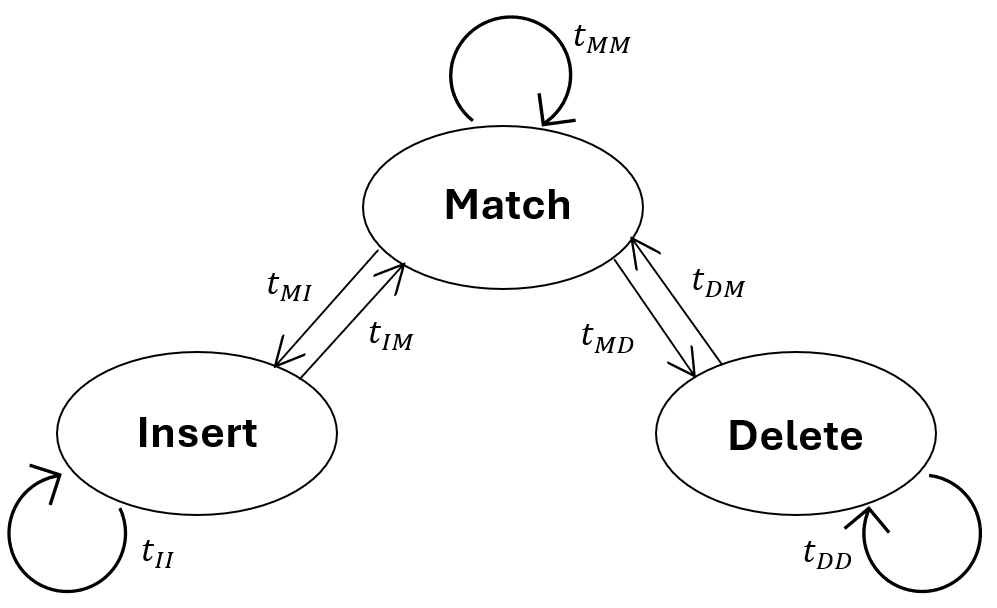
\includegraphics[width=0.7\linewidth]{figure/state.png}
    \caption{State diagram of Pair-HMM}
    \label{fig:state diagram}
\end{figure}

\begin{table}[h]
    \centering
    \begin{tabular}{cccccc}
    \multicolumn{1}{c}{Read:} & A & C & C & G & - \\
    \multicolumn{1}{c}{Haplotype:} & A & C & - & G & A \\
    \multicolumn{1}{c}{Hidden state:} & M & M & I & M & D \\
    \end{tabular}
    \caption{A example of Pair-HMM generating the hidden-state}
    \label{tab:hidden state}
\end{table}
Therefore, the probability \textit{P} of this pair of read and haplotype sequence alignment happens can be computed as 
\begin{align*}
P &= e(A,A) \times\ t_{M,M} \times\ e(C,C) \times\ t_{M,I} \times\ e(C,-) \times\ t_{I,M} \\
  &\quad\times\ e(G,G) \times\ t_{M,D} \times\ e(-,A)
\end{align*}

In this equation, \textit{e(alphabet,alphabet)} typically represents the "emission probability". The emission probability is the probability of observing a particular visible alphabet given a specific state in the model. \textit{$t_{state,state}$} is the transition probability which is the probability of moving from one state to another as the mentioned above.

The Pair-HMM Forward Algorithm is one of the most accurate methods for sequence alignment~\cite{Shanshan1,EnliangLi1}. It is a computational method used within the context of the Pair-HMM to calculate the probability of an observed sequence alignment without any conditionals. The final alignment probability is the most critical piece of information for understanding how well two sequences align under the given model.

The Pair-HMM Forward Algorithm is shown as in Algorithm 1. \textit{M}, \textit{I} and \textit{D} are the forward matrices used to store the probabilities of the sequences aligning through matching, insertion, or deletion. \textit{m} and \textit{n} are the length of the read \textit{R} and the haplotype \textit{H}. $e_{i,j}$ represents the Emission Probability which is the probability of current State emitting the given pair character($Read_{i},Haplotype_{j}$).  $t_{A,B}$ represents the Transition probability which is the probability of transitioning from state A to state B, as the mention above.
The Pair-HMM Forward Algorithm used dynamic programming technique to iterate through all possible alignments between the read and reference sequence. It can be broken down into four key steps.

(1) \textbf{Initialization:} In Line 1, The algorithm initializes three forward matrices: Match (\textit{M}), Insert (\textit{I}), and Delete (\textit{D}). Set the values for the first row of the matrices, where $M_{0,j}= I_{0,j} = 0 $ and $D_{0,j} = 1 / n $ for $1 <= j <= n$. This accounts for the possibility of starting with free deletions in the haplotype. 

(2) \textbf{Iterative Update:} In Line 2 and 3, the outer loop iterates through each position \textit{i} in the read sequence (from 1 to m) and the inner loop iterates through each position \textit{j} in the haplotype sequence (from 1 to n). This nested loop structure allows the algorithm to consider every possible alignment between subsequences of the read and haplotype.

(3) \textbf{Updating:} In Line 4, 5 and 6, update the forward matrices with the corresponding cells. The Match state also needs to consider the emission probability because it represents the likelihood of aligning the current nucleotide in the read with the current nucleotide in the haplotype. 

(4) \textbf{Calculates likelihood:} In Line 7, after completing the nested loops, the algorithm calculates the total likelihood of observing the read sequence given the haplotype by summing the final entries in the Match and Insert matrices : $\sum_{j=1}^{n} (M_{m,j} + I_{m,j})$ \textbf{for} $1 \leq j \leq n$.\newline
However, along with accurate results comes a huge amount of computation. The pair HMM Forward Algorithm is computationally intensive especially  processing large-scale genomic data. Moreover, with the growing DNA sequencing data, the overhead of computation is becoming heavier and heavier. \newline
% 定義自定義命令以隱藏end for
\algtext*{Procedure}
\algtext*{EndFor}
\algtext*{EndProcedure}

\begin{algorithm}
\caption{Pseudocode for Pair-HMM Forward Algorithm}
\begin{algorithmic}[1]
\Procedure\textbf{Pair-HMM Forward Algorithm}
\State Initialize Matrices: $M_{0,j} = I_{0,j} = 0$ and $D_{0,j} = \frac{1}{n}$ \textbf{for} $1 \leq j \leq n$
\For{$i = 1$ \textbf{to} $m$}
    \For{$j = 1$ \textbf{to} $n$}
        \State $M_{i,j} \gets e_{Read_{i},Haplotype_{j}} (t_{MM} M_{i-1,j-1}  + t_{IM} I_{i-1,j-1}  +  t_{DM} D_{i-1,j-1})$
        \State $I_{i,j} \gets t_{MI} M_{i-1,j}  + t_{II} I_{i-1,j} $
        \State $D_{i,j} \gets t_{MD} M_{i,j-1} + t_{DD} D_{i,j-1} $
    \EndFor
\EndFor
\State \textbf{return }$\sum_{j=1}^{n} (M_{m,j} + I_{m,j})$ \textbf{for} $1 \leq j \leq n$
\EndProcedure
\end{algorithmic}
\end{algorithm}

\section{Motivation}
In DNA sequence alignment, the use of DNA sequence profiles is crucial due to sequencing errors and the common presence of single nucleotide polymorphisms (SNPs) in humans ~\cite{Xuhua,Dimitrios}. Sequencing errors cause the sequenced DNA to differ from the actual DNA sequence ~\cite{sequencingError}. To address these errors, it is essential to incorporate a probabilistic model into the alignment algorithm. By representing each base as a probability, the alignment process can better accommodate the uncertainties in the sequencing results, resulting in more accurate alignments. SNPs are the most common type of genetic variation among individuals of the same species, where a single base pair differs between individuals ~\cite{Xuhua}. SNPs are common in the human genome and must be considered during sequence alignment. Utilizing DNA sequence profiles enables each position in the sequence to be represented as a probability distribution, capturing the variability caused by SNPs. This probabilistic representation helps the alignment process to more precisely match sequences by considering these common variations.

In addition to utilizing profiles for more precise analysis, the speed of computation is also a crucial point. As previously mentioned, with the increasing volume of DNA sequencing data, the computational burden of pair HMM Forward Algorithm grows heavier. Therefore, we have opted to leverage CUDA to harness the benefits of parallel computing on GPUs to achieve accelerated performance.

\section{CUDA}
CUDA (Compute Unified Device Architecture) is a parallel computing platform and programming model developed by NVIDIA~\cite{CUDA}. It enables developers to utilize NVIDIA GPUs for general-purpose computing, often referred to as GPGPU (General-Purpose computing on Graphics Processing Units). CUDA allows developers to write code in programming languages such as C, C++, which can then be executed on GPUs to perform large-scale parallel computations.

Three of the main advantages about CUDA : (1) Parallel Execution: CUDA provides an environment through which developers can access GPU hardware via a programming interface, enabling them to run compute-intensive tasks directly on the GPU. (2) Efficient Memory Management: CUDA offers efficient memory management functions to transfer data between the host and device. Makes it easier for developers to design their kernel to achieve their goals in an efficient way. (3) Scalability: CUDA allows developers to write code that can efficiently handle increasing problem sizes and leverage the full computational power of the GPU. By properly managing threads, memory, streams, and utilizing multiple GPUs, CUDA applications can achieve significant performance improvements for large-scale and complex computations.  

The figure \ref{fig:core component} provides a visual representation of the core components of CUDA architecture, illustrating the relationship between the host (CPU) and the device (GPU) ~\cite{CUDA}. (1) \textbf{Host}: The host represents the CPU, which is responsible for launching and managing the execution of CUDA kernels on the GPU. Besides, the host prepares the data, transfers it to the device and initiates the kernel execution. (2) \textbf{Device}: The device represents the GPU, which executes the computational kernels. The GPU consists of several multiprocessors, each containing many cores capable of executing hundred of threads concurrently. (3) \textbf{Kernel}: Kernel is a function written in CUDA C/C++ that runs on the GPU. When a kernel is launched, it is executed by a large number of parallel threads on the GPU. (4) \textbf{Grid}: The grid is a collection of blocks. In this figure, Grid 1 is shown as containing multiple blocks. Each grid corresponds to a kernel launch, and all blocks within a grid execute the same kernel function. The grid structure allows for organizing computations over large datasets. (5) \textbf{Block}: Block is a group of threads that can cooperate by sharing data through shared memory and synchronizing their execution. Each block is identified by its indices, such as Block (0,0), Block (0,1), and so on. Blocks are scheduled on different multiprocessors of the GPU. (6) \textbf{Thread}: Thread is the smallest unit of execution in CUDA. Each thread within a block has a unique thread index. Threads within the same block can communicate and synchronize with each other, making it possible to solve complex problems efficiently. The figure illustrates the thread layout within Block (1,1), showing threads indexed from Thread (0,0) to Thread (2,2).

\begin{figure}[h]
    \centering
    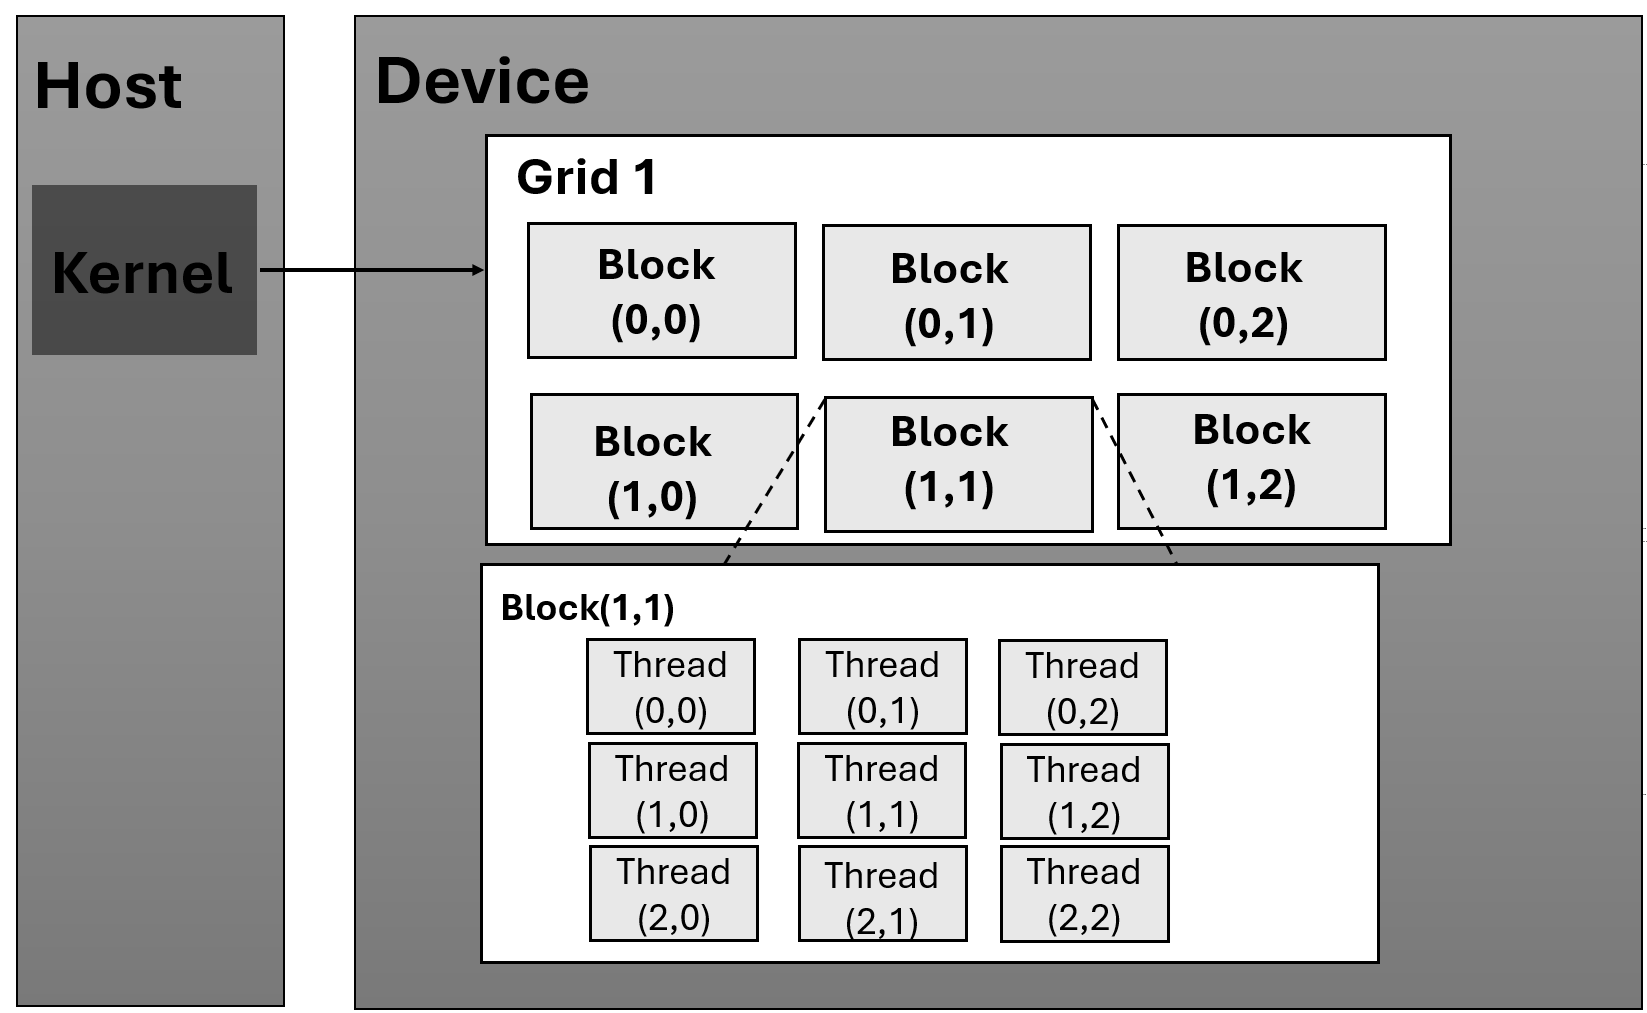
\includegraphics[width=1\linewidth]{figure/grid_block_thread.png}
    \caption{CUDA core component}
    \label{fig:core component}
\end{figure}

\chapter{Related Work}
Previous studies have attempted to enhance the performance of the pair HMM Forward Algorithm in various ways. Shanshan Ren et al.~\cite{Shanshan} focused on two GPU-based implementations: (1) \textbf{Intertask}: Each thread independently executes the algorithm on a different pair of sequences (read haplotype), meaning each thread runs the Pair-HMM Forward Algorithm independently, requiring synchronization with other threads. (2) \textbf{Intratask}: This involves breaking down the computation within a single instance of the algorithm into smaller subtasks that can be executed concurrently by multiple threads. For instance, segments of the dynamic programming matrix can be computed in parallel, but the parallelism must synchronize at specific points to ensure that data dependencies are respected. Enliang Li et al.~\cite{EnliangLi} utilize GPU with Anti-Diagonal Parallelization to accelerate the Pair-HMM Forward algorithm which is a common acceleration technique for dynamic programming with GPU parallel computing. Besides, they also use shared memory to store intermediate data prevent from the expensive communication between host and device. Subho S. Banerjee et al.~\cite{Subho} and Sitao Huang et al.~\cite{Sitao} implement the Pair-HMM Forward Algorithm on a Field-Programmable Gate Array (FPGA) with enhanced data forwarding strategies and customized computation routines for improved performance.

However, those studies all focus on DNA sequence, not DNA sequence profile. As noted above, DNA sequence profile is important to obtain a more precise analysis. Therefore, we leverage the advantages of the previous GPU-based accelerating method to develop an improved version of the Pair-HMM forward algorithm for DNA sequence profiles, which is suitable for large-scale genomic data. We will discuss the difference in the pair-HMM forward algorithm when the profile is considered in the next chapter.

\chapter{Profile}
The profile approach considers that the input read has a probability distribution over multiple nucleotides, rather than being a single, deterministic nucleotide sequence \cite{Emad}. This means that each position in the read is represented by a vector of probabilities, indicating the likelihood of observing each nucleotide (A, C, G, T) at that position.

Table \ref{tab:profile} shows an example of the read \textbf{ACCGT} represented in profile form. Each cell in the matrix represents the probability of observing a specific nucleotide at a given position in the read. For instance, the probability of observing an `A' at the first position is 0.8, while the probability of observing a `C' at the second position is 0.7, and so on.

\begin{table}[h]
    \centering
    \begin{tabular}{c|ccccc}
         & A & C & C & G & T \\
        \hline
        A & \textbf{0.8} & 0 & 0.1 & 0.1 & 0 \\
        C & 0.1 & \textbf{0.7} & \textbf{0.9} & 0 & 0.05 \\
        G & 0.1 & 0.15 & 0 & \textbf{0.7} & 0 \\
        T & 0 & 0.15 & 0 & 0.2 & \textbf{0.95} \\
    \end{tabular}
    \caption{The example of profile form}
    \label{tab:profile}
\end{table}

This probabilistic representation significantly impacts the emission probabilities in a Hidden Markov Model (HMM) used for sequence alignment. In traditional HMMs, emissions are typically based on the most likely nucleotide at each position. However, when using a profile representation, the emission probability must consider the entire probability distribution over possible nucleotides ~\cite{Profile}.

The concept of Profile Emission Probability is crucial in this context. It calculates the probability of the observed read given the underlying state in the HMM, taking into account the entire distribution of possible nucleotides at each position. This ensures that the model accurately reflects the uncertainties in the sequence data, which is particularly important in noisy or error-prone data sets, such as those generated by high-throughput sequencing technologies.

The algorithm 2 illustrates the process of calculating the Profile Emission Probability. This algorithm aggregates the probabilities of emitting each possible nucleotide from the state, weighted by the observed probabilities in the read. To be more detailed, this function iterates over each nucleotide base (A, C, G, T) and calculates the total emission probability by summing the product of the read probability and the emission matrix value for the given state. This approach ensures that all possible nucleotide emissions are considered, weighted by their respective probabilities, providing a comprehensive emission probability that accurately reflects the read's profile.
\vspace{0.5cm} % Add vertical space before the algorithm
\begin{algorithm}
\caption{Calculate Profile Emission Probability}
\begin{algorithmic}[1]
\Function{CalculateProfileEmission}{$\text{readProb}, \text{haplotype}, \text{emissionMatrix}, \text{state}$}
    \State $\text{totalProb} \gets 0$ 
    \For{each base $i$ in the set $\{A, C, G, T\}$}
            \State $\text{totalProb} \gets \text{totalProb} + (readProb_{i} \times emissionMatrix_{state,i,haplotype})$ 
    \EndFor
    \State \Return $\text{totalProb}$ 
\EndFunction
\end{algorithmic}
\end{algorithm}
\vspace{0.5cm} % Add vertical space before the algorithm
\[
\text{totalProb} = \sum_{i \in \{A,C,G,T\}} (\text{readProb}_i \times \text{emissionMatrix}_{\text{state},i,\text{haplotype}})
\]
\newpage
Algorithm 3 presents the pseudocode of the Pair-HMM Forward Algorithm with Profile Emissions. The key difference between this version and the traditional Pair-HMM Forward Algorithm lies in the update process for the forward matrices.When updating the \textbf{Match} and \textbf{Insert} matrices, the algorithm incorporates the profile emission probabilities. This means that the entire probability distribution over possible nucleotides at each position in the read is considered. This is crucial for accurately modeling the uncertainty and variability in sequencing data.In contrast, for the \textbf{Delete} matrix, the nucleotide in the read sequence $read_{i}$ is a gap. Therefore, the profile emission probabilities are not needed for the Delete state.
\vspace{0.5cm} % Add vertical space before the algorithm
\begin{algorithm}
\caption{Pseudocode for Pair-HMM Forward Algorithm with Profile Emissions}
\begin{algorithmic}[1]
\Procedure\textbf{Pair-HMM Forward Algorithm with Profile Emissions}
\State Initialize Matrices: $M_{0,j} = I_{0,j} = 0$ and $D_{0,j} = \frac{1}{n}$ \textbf{for} $1 \leq j \leq n$
\For{$i = 1$ \textbf{to} $m$}
    \For{$j = 1$ \textbf{to} $n$}
        \State $e_{M_{i,j}} \gets \text{CalculateProfileEmission}(read_{i}, haplotype_{j}, emissionMatrix, Match)$
        \State $e_{I_{i,j}} \gets \text{CalculateProfileEmission}(read_{i-1}, gap, emissionMatrix, Insert)$
        \State $M_{i,j} \gets e_{M_{i,j}} (t_{MM} M_{i-1,j-1}  + t_{IM} I_{i-1,j-1}  +  t_{DM} D_{i-1,j-1})$
        \State $I_{i,j} \gets e_{I_{i,j}} (t_{MI} M_{i-1,j}  + t_{II} I_{i-1,j} )$
        \State $D_{i,j} \gets (t_{MD} M_{i,j-1} + t_{DD} D_{i,j-1} )$
    \EndFor
\EndFor
\State \textbf{return }$\sum_{j=1}^{n} (M_{m,j} + I_{m,j})$ \textbf{for} $1 \leq j \leq n$
\EndProcedure
\end{algorithmic}
\end{algorithm}
\vspace{0.5cm} % Add vertical space before the algorithm
\newline
By considering the entire probability distribution over possible nucleotides at each position, the algorithm effectively handles the uncertainties inherent in high-throughput sequencing data. This should result in more reliable and meaningful alignments.

\chapter{Methods}
In this chapter, we will introduce the implementation details of our gpu-accelerated version.
\section{Workflow}
Figure \ref{fig:workflow} illustrates the workflow for Host and Device, which can be divided into several steps.
(1) \textbf{Initialization on Host}: Initialize the required data structures and parameters on the host (CPU). This involves reading the sequence data, preparing the emission and transition matrices, and allocating memory for the forward matrices. (2) \textbf{Memory Allocation on Device}: Allocate memory on the device (GPU) for the read probability matrix, haplotype sequence, emission matrix, transition matrix, and the forward matrix for Match, Insert, and Delete states. (3) \textbf{Data Transfer from Host to Device}: Transfer the initialized data from the host to the device memory to ensure that the GPU has all the necessary data for computation. (4) \textbf{Kernel Launch}: Launch the CUDA kernel(s) to execute the Pair-HMM Forward Algorithm computations. The kernels will update the forward matrices based on the profile emission probabilities, transition probabilities and previous cells. (5) \textbf{Data Transfer from Device to Host}: Transfer the results from the device back to the host memory. This enables the host to access the computed results for further processing or output.
\begin{figure}
    \centering
    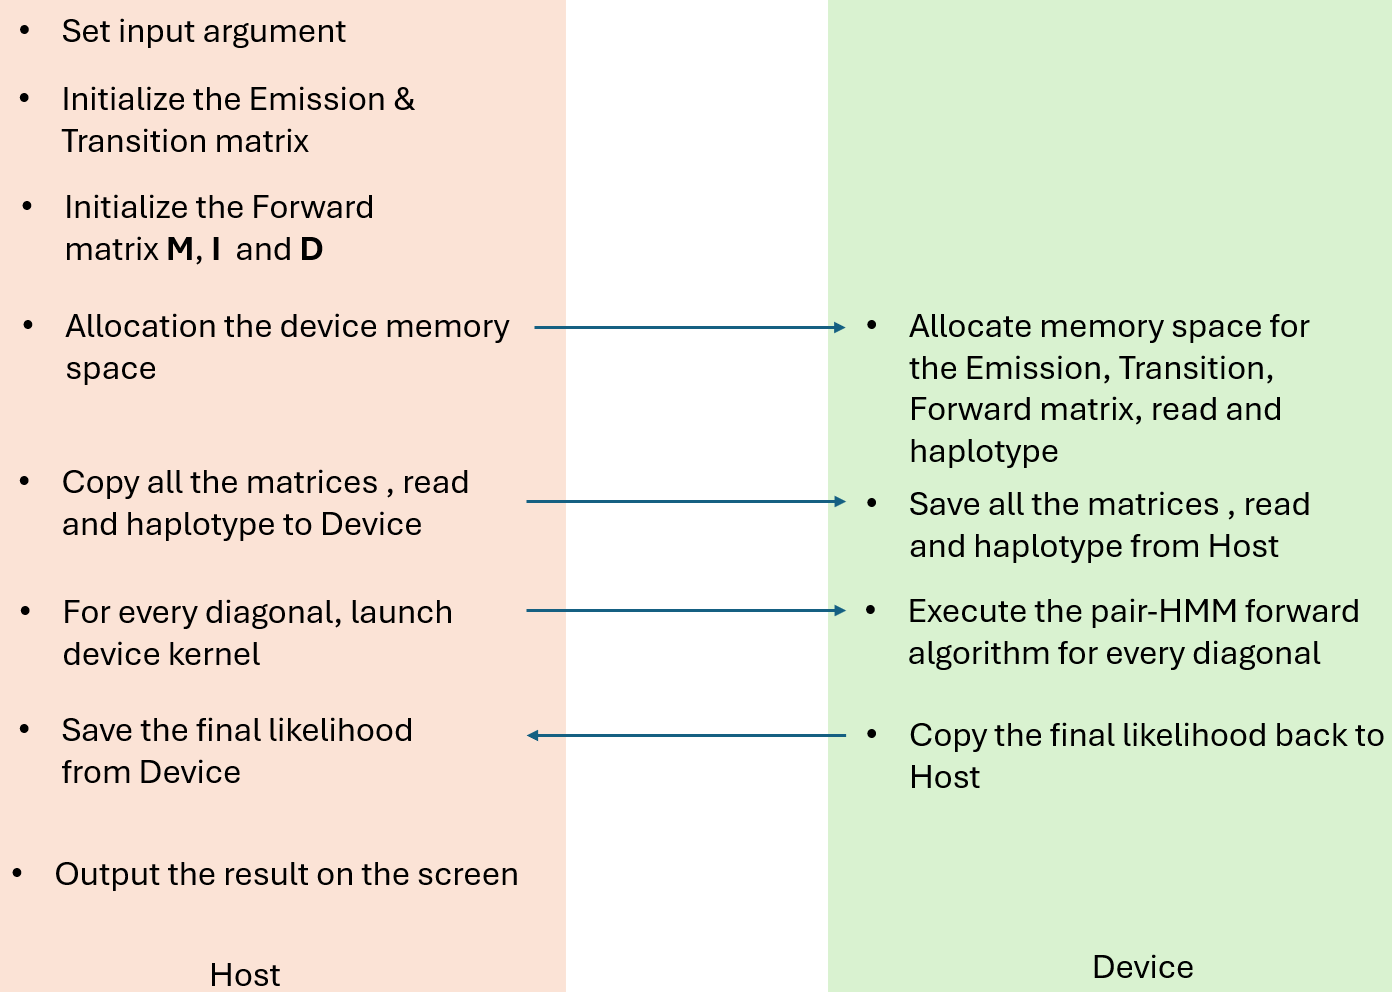
\includegraphics[width=1.1\linewidth]{figure/Host-Device.png}
    \caption{Workflow for Host and Device}
    \label{fig:workflow}
\end{figure}

\section{Flatten}
In CUDA, flattening multi-dimensional arrays into a one-dimensional array is a common method. This approach simplifies memory access patterns, enhances performance, and aligns better with CUDA memory model. CUDA supports only one-dimensional (1D) linear memory addressing. While CUDA kernels can work with multi-dimensional data, such as 2D or 3D arrays, they need to convert these data structures into a linear memory space. Flattening these structures into a 1D array makes it easier to manage and access memory using a single index calculation. In this way, we could improve Memory Coalescing. Memory coalescing is a mechanism that allows for efficient memory access by combining multiple memory operations into a single transaction. For best performance, neighboring threads should access contiguous memory addresses. Flattening multi-dimensional arrays ensures that adjacent elements in the array are stored contiguously in memory, which enhances the likelihood of memory coalescing and improves overall memory bandwidth utilization. Hence, before we transfer the forward matrices from host to device, we should flatten them into 1D arrays to have efficient memory access.

\begin{figure}[h]
    \centering
    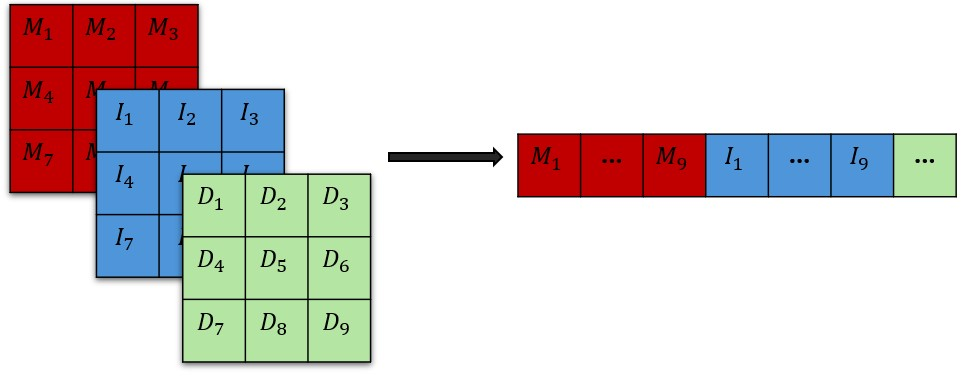
\includegraphics[width=1\linewidth]{figure/Flatten.jpg}
    \caption{The flatten of Forward Matrix}
    \label{fig:flatten}
\end{figure}


\section{Log-Scale}
The use of log-scale in computational algorithms helps to mitigate numerical underflow and overflow issues. In the Pair-HMM Forward Algorithm, probabilities resulting in exceedingly small products when multiplied together in long sequences. Direct computation with these small probabilities can lead to numerical underflow, where values are rounded to zero, causing inaccuracies in the results. By representing probabilities in the logarithmic domain, the multiplication of probabilities is converted into addition, and division into subtraction. This not only stabilizes the numerical computations but also simplifies the mathematical operations.

Another critical technique is the use of the log-sum-exp trick, which is a technique to compute the logarithm of a sum of exponential in a numerically stable way. The log-sum-exp function is defined as follows:

\[
\log \sum_{i=1}^{n} e^{x_i}
\]

To compute this expression in a numerically stable way, we can use the following equivalent formula:

\[
\log \sum_{i=1}^{n} e^{x_i} =   \log \sum_{i=1}^{n} (e^{x_i-\alpha} e^{\alpha})
                            =    \alpha + \log \sum_{i=1}^{n} e^{x_i - \alpha}
\]

where \(\alpha = \max(x_1, x_2, \ldots, x_n)\).

Direct computation of \(\sum_{i=1}^{n} e^{x_i}\) can result in numerical instability if some of the \(x_i\) values are very large or very small. This can lead to overflow or underflow in the exponentiation step. To enhance numerical stability, we factor out the maximum value, \(\alpha\), from the exponentials. This is achieved by subtracting \(\alpha\) from each \(x_i\) inside the exponential, which ensures that all exponents are non-positive and hence no overflow occurs.

\subsection{Example}

Suppose we have \(x_1 = 1000\), \(x_2 = 1001\), and \(x_3 = 1002\):

\begin{enumerate}
    \item \textbf{Find Maximum \(\alpha\)}:
    \[
    \alpha = \max(1000, 1001, 1002) = 1002
    \]
    
    \item \textbf{Compute the Sum of Exponentials with Subtracted Maximum}:
    \[
    \sum_{i=1}^{3} e^{x_i - \alpha} = e^{1000 - 1002} + e^{1001 - 1002} + e^{1002 - 1002} = e^{-2} + e^{-1} + e^{0}
    \]
    
    \item \textbf{Evaluate}:
    \[
    e^{-2} + e^{-1} + e^{0} \approx 0.1353 + 0.3679 + 1 = 1.5032
    \]
    
    \item \textbf{Apply Log and Add Maximum}:
    \[
    \log \sum_{i=1}^{3} e^{x_i} = \alpha + \log (1.5032) = 1002 + \log (1.5032) \approx 1002 + 0.4076 = 1002.4076
    \]
\end{enumerate}

Implementing the pair-HMM forward algorithm in log-scale ensures that the algorithm remains robust and accurate even when dealing with long sequences and small probabilities. By using the log-sum-exp trick, we can ensure that our calculations remain stable and accurate, even when dealing with extreme values. This section provides an in-depth look at how log-scale transformations and the log-sum-exp trick are applied within the algorithm, demonstrating their importance in achieving reliable and meaningful results in sequence alignment tasks.

\section{Anti-Diagonal Parallelism}
Anti-diagonal parallelism is a widely used parallel processing technique in dynamic programming algorithms, such as the pair-HMM forward algorithm. This technique leverages the inherent data dependencies in these algorithms to enable concurrent computation of multiple cells, significantly improving performance. In the next subsection, we will explain why the pair-HMM can be implemented with anti-diagonal parallel technique by discussing its data dependency.
\subsection{Data Dependency}
The computation of pair-HMM forward algorithm indicates each cell in the forward matrices (\textit{M}, \textit{I}, and \textit{D}) depends on the values of previously computed cells.
\begin{itemize}
    \item $M_{i,j}$ depends on $M_{i-1,j-1}$, $I_{i-1,j-1}$, and $D_{i-1,j-1}$.
    \item $I_{i,j}$ depends on $M_{i-1,j}$ and $I_{i-1,j}$.
    \item $D_{i,j}$ depends on $M_{i,j-1}$ and $D_{i,j-1}$.
\end{itemize}
\begin{figure}[h]
    \centering
    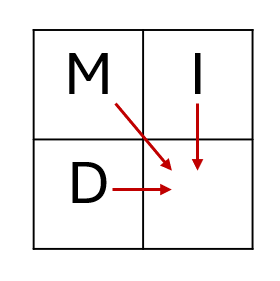
\includegraphics[width=0.5\linewidth]{figure/data-dependency.png}
    \caption{The data dependency for pair-HMM forward algorithm}
    \label{fig:data dependency}
\end{figure}
Therefore, for any cell $M_{i,j}$ on the same anti-diagonal $i+j=k$, the dependencies come from cells on the previous anti-diagonal $i+j=k-2$. For $I_{i,j}$ and $D_{i,j}$ on the same anti-diagonal $i+j=k$ the dependencies come from cells on the previous anti-diagonal $i+j=k−1$.

The figure \ref{fig:dependency diagram} is the dependency diagram for the pair-HMM forward algorithm. The yellow arrows indicate dependencies on blue cells. As we can see, the update of blue cells only depends on red cells for Match matrix and depends on green cells for Insert and Delete matrices. Consequently, we can infer that those blue cells are independent of each other. Generally speaking, the update on the same anti-diagonal can be executed in parallel.
\begin{figure}[h]
        \centering
        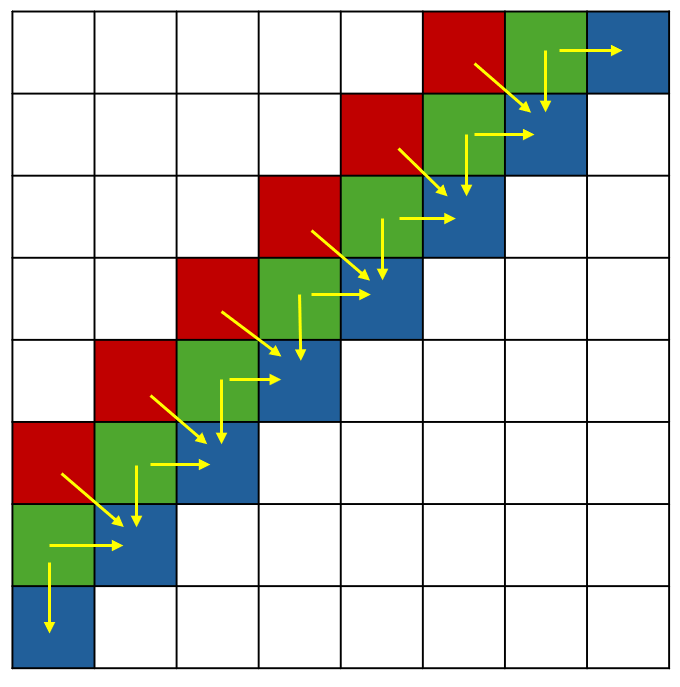
\includegraphics[width=0.7\linewidth]{figure/anti-diagonal.png}
        \caption{Dependency diagram}
        \label{fig:dependency diagram} 
\end{figure}
\newpage
The Algorithm 4 presents the pseudocode for anti-diagonal parallelization of pair-HMM forward algorithm with profile emissions. This approach parallelizes the update of cells on the same anti-diagonal $i+j=k$ through $k$ from $2$ to $n+m$. The first n iterates the update of the upper left half matrix, while the last $n+1$ to $n+m$ iterates update the lower right half matrix. The index is controlled by the $threadIdx.x$ and $k$. If the index is within the matrix, the thread will perform the updating.
\vspace{0.5cm}
\begin{algorithm}[h]
\caption{Pseudocode for Anti-Diagonal Parallelization of Pair-HMM Forward Algorithm with Profile Emissions}
\begin{algorithmic}[1]
\Procedure{Pair-HMM Forward Algorithm with Anti-Diagonal Parallelization}{}
\State Initialize Matrices: $M_{0,j} = I_{0,j} = 0$ and $D_{0,j} = \frac{1}{n}$ \textbf{for} $1 \leq j \leq n$
\For{each anti-diagonal $k$ from $2$ to $m+n$}
    \State \textbf{parallel for} each $(i, j)$ on anti-diagonal $i+j=k$ \textbf{do}
    \State $i$ \gets $k$ \minus $threadIdx.x$
    \State $j$ \gets $threadIdx.x$
    \If{$i > 0$ and $i \leq m$ and $j > 0$ and $j \leq n$}
        \State $e_{M_{i,j}} \gets \text{CalculateProfileEmission}(read_i, haplotype_j, emissionMatrix, Match)$
        \State $e_{I_{i,j}} \gets \text{CalculateProfileEmission}(read_{i-1}, gap, emissionMatrix, Insert)$
        \State $M_{i,j} \gets e_{M_{i,j}} (t_{MM} M_{i-1,j-1} + t_{IM} I_{i-1,j-1} + t_{DM}  D_{i-1,j-1})$
        \State $I_{i,j} \gets e_{I_{i,j}}  (t_{MI}  M_{i-1,j} + t_{II}  I_{i-1,j})$
        \State $D_{i,j} \gets t_{MD}  M_{i,j-1} + t_{DD}  D_{i,j-1}$
    \EndIf
\EndFor

\State \Return $\sum_{j=1}^{n} (M_{m,j} + I_{m,j})$
\EndProcedure
\end{algorithmic}
\end{algorithm}

By using anti-diagonal parallel optimization, we can reduce the time complexity from $O(n*m)$ to $O(n+m)$, which is a significant advancement in reducing computation time if the read and haplotype are long sequence. However, the space complexity remains $O(n*m)$, resulting in the storage of the entire forward matrix. Therefore, we will introduce our method to reduce the space complexity in the following section.
\newpage
\section{Anti-Diagonal Rolling}
In order to avoid storing the whole forward matrix, we implement the anti-diagonal rolling technique, which is an common-used optimization technique in dynamic programming algorithm. In the former section, we have discussed about the data dependency of pair-HMM forward algorithm. We already know that the update of the cells on anti diagonal $i+j=k$ only depend on the previous anti-diagonal $i+j=k-1$ and $i+j=k-2$. Therefore, instead of storing the entire forward matrix, we only store the last two anti-diagonal sequence for the computation and record the current anti-diagonal cell for the next anti-diagonal iterate. 

Figure \ref{fig:The example of Anti-Diagonal Rolling} shows an example where we only store the red cells and green cells for the update of the blue cells. After the updates of the blue cells are all finished, we perform the rolling step to shift the current anti-diagonal values to the previous anti-diagonal storage and update the current anti-diagonal storage for the next computation.
Figure \ref{fig:The process of anti-diagonal rolling} illustrates the process of anti-diagonal rolling in more detail. Initially, the cells from the red (pre-previous), green (previous), and blue (current) anti-diagonals are stored. After the blue cells are updated, they are used to compute the yellow cells in the next anti-diagonal. The rolling process is as follows:
(1) The values from the current anti-diagonal (blue cells) are shifted to the previous anti-diagonal storage.
(2) The values from the previous anti-diagonal (green cells) are shifted to the pre-previous anti-diagonal storage.
(3) The current anti-diagonal storage is then updated with the newly computed values (yellow cells).

This anti-diagonal rolling technique ensures that only a small and fixed amount of memory is used. By storing and updating only the necessary anti-diagonals, we efficiently manage memory usage while maintaining the correctness and performance of the algorithm. In the discussion of the space complexity aspect, the space complexity drops from $O(n*m)$ to $O(max(n,m))$ depend on the length of the read and haplotype.

\begin{figure}[h]
    \centering
    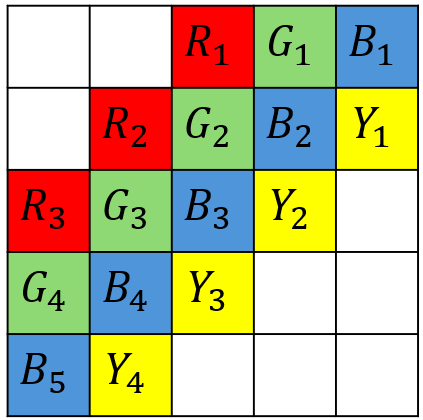
\includegraphics[width=0.5\linewidth]{figure/rolling-example.png}
    \caption{The example of Anti-Diagonal Rolling}
    \label{fig:The example of Anti-Diagonal Rolling}
\end{figure}
\begin{figure}[h]
    \centering
    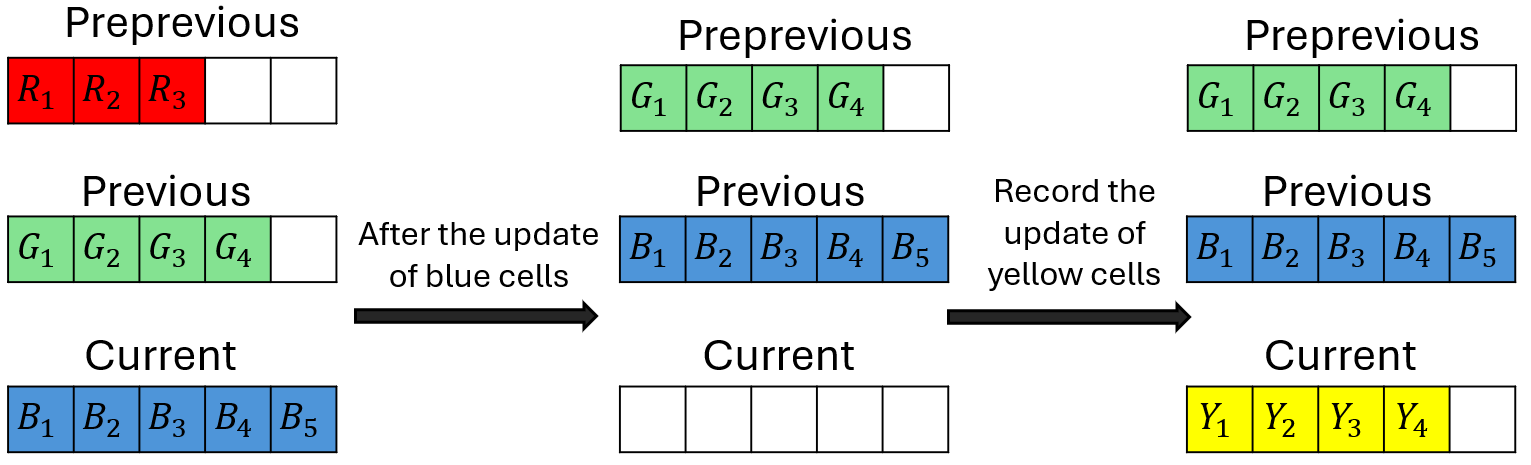
\includegraphics[width=1.1\linewidth]{figure/theProcessOfAnti-DiagonalRolling.png}
    \caption{The process of Anti-Diagonal Rolling}
    \label{fig:The process of anti-diagonal rolling}
\end{figure}


After implementing anti-diagonal rolling into our algorithm, a few changes have been made. The first change is that the update now depends on the preprevious, previous and current matrices. The second modification is the addition of the rolling step in lines 17-19, which enhances the algorithm's efficiency by reusing the same memory space instead of storing the entire forward matrix. The final change is a consequence of the second adjustment. Since we no longer have the complete forward matrix, we must calculate the likelihood within the algorithm each time it reaches the bottom row, as shown in lines 14-15.
\newpage
\begin{algorithm}[h]
\caption{Pseudocode for Anti-Diagonal Parallelization and Rolling of Pair-HMM Forward Algorithm with Profile Emissions}
\begin{algorithmic}[1]
\Procedure{Pair-HMM Forward Algorithm with Anti-Diagonal Parallelization and Rolling}{}
\State Initialize all the needed Matrices
\State Initialize $likelihood \gets0$
\For{each anti-diagonal $k$ from $2$ to $m+n$}
    \State \textbf{parallel for} each $(i, j)$ on anti-diagonal $i+j=k$ \textbf{do}
    \State $i$ \gets $k - threadIdx.x$
    \State $j$ \gets $threadIdx.x$
    \If{$i > 0$ and $i \leq m$ and $j > 0$ and $j \leq n$}
        \State $e_{M_{i,j}} \gets \text{CalculateProfileEmission}(read_i, haplotype_j, emissionMatrix, Match)$
        \State $e_{I_{i,j}} \gets \text{CalculateProfileEmission}(read_{i-1}, gap, emissionMatrix, Insert)$
        \State $currM_{i} \gets e_{M_{i,j}} \times (t_{MM} \times preprevM_{i-1} + t_{IM} \times preprevI_{i-1} + t_{DM} \times preprevD_{i-1})$
        \State $currI_{i} \gets e_{I_{i,j}} \times (t_{MI} \times prevM_{i-1} + t_{II} \times prevI_{i-1})$
        \State $currD_{i} \gets t_{MD} \times prevM_{i} + t_{DD} \times prevD_{i}$
    \EndIf
    \If{$i==m$}
        \State $likelihood \gets likelihood + currM_{i} + currI_{i}$
    \EndIf
\State $prevprev \gets prev$
\State $prev \gets curr$
\State $curr \gets 0$

\EndFor
\State \textbf{return }likelihood
\EndProcedure
\end{algorithmic}
\end{algorithm}

By incorporating anti-diagonal rolling, Algorithm 5 optimizes memory usage and enhances the computational efficiency of the Pair-HMM Forward Algorithm with Profile Emissions. This makes it more suitable for large-scale applications where memory resources are a critical concern.

\chapter{Results}

\section{Benchmark}
To evaluate the performance of our GPU-based accelerated Pair-HMM Forward Algorithm for DNA sequence profile alignment, we conducted a series of experiments using a CPU version implemented in C++ as the benchmark. We generated random read and haplotype sequences with various numbers of base pairs: $100$, $1000$,  $10,000$, $100,000$. Additionally, we compared the performance of fixed blocks and dynamic blocks in the GPU-based implementation to check the improved effect of dynamic blocks allocation.

\section{Experimental Setup}
The experiments were conducted on a computer with an Intel i7-12700 desktop processor, which features 12 cores, 20 threads, and operates at 2.1 GHz by default. The GPU of the computer is a TUF Gaming GeForce RTX™ 3080 graphics card.

\section{Configuration setting}
Before comparing with the benchmark, we have to find out the best configuration for our GPU-based implementation. We would compare all combinations of 32, 64, 128, 256, fixed blocks and thread in different numbers of base pairs(bp). Besides, we implement dynamic block technique to compare with fixed block, which is a relatively rare technique to utilize.
\subsection{Dynamic Block}
In the field of CUDA programming, dynamic block is a technique used to efficiently distribute the computational workload across available GPU resources. By dynamically determining the number of blocks required based on the size of the problem, we can optimize the performance and ensure that the GPU is utilized effectively.
In the pair-HMM forward algorithm, the computation is distributed along the anti-diagonals of the forward matrix. The number of elements in each anti-diagonal varies, and thus, the computational load also varies. To handle this variation efficiently, we use dynamic block allocation. The following is the mathematical formula for dynamic block allocation.
\[
\ blocksNum = \left\lfloor \frac{(elementsInDiag + threadsNum- 1) }{threadsNum} \right\rfloor
\]
We will explain the purpose of every parameter in this formula. First,  $\left\lfloor.\right\rfloor$ : When performing integer division, any fractional part of the result is discarded, effectively rounding down to the nearest whole number. This operation is known as taking the floor of the division result. Hence, we need the floor to represent the action of integer division. Second, \textbf{elementsInDiag} : The total number of elements along the anti-diagonal. As mentioned above, the computation is distributed along the elements of anti-diagonals. Therefore, we need the \textit{elementsInDiag} in the formula to adjust through the computation size for determining the number of blocks. Third, \textbf{threadsNum} : The number of threads per block. \textit{ThreadsNum in the denominator} determines the granularity of the parallel computation. Each block contains a fixed number of threads (threadsNum), which collaborate to compute the values along the anti-diagonal.   As for \textit{ThreadsNum in the numerator} is used to prevent from the \textit{blocksNum} becoming zero when the \textit{elementsInDiag} is less than \textit{threadsNum}. Last, \textbf{-1}, in the case of exact division (e.g., elementsInDiag = threadsNum), the \textbf{-1} ensures the minimization of the number of blocks, preventing the waste of computational resources. The following is an example of an exact division. In this example, we only need one block to compute perfectly. With \textbf{-1}, we can generate exactly the number of blocks we need.

\textbf{Example: elementsInDiag = 4, threadsNum = 4}

\noindent
**Formula with \(-1\)**:
\[
\text{blocksNum} = \left\lfloor \frac{4 + 4 - 1}{4} \right\rfloor = \left\lfloor \frac{7}{4} \right\rfloor = \left\lfloor 1.75 \right\rfloor = 1
\]

\noindent
**Formula without \(-1\)**:
\[
\text{blocksNum} = \left\lfloor \frac{4 + 4}{4} \right\rfloor = \left\lfloor \frac{8}{4} \right\rfloor = \left\lfloor 2 \right\rfloor = 2
\]
\newpage
The table \ref{tab:100} shows the comparison of the execution time with 100bp read and haplotype in milliseconds.
100bp is the average length of the NGS data. The experiment indicates that the block size 32 and the thread size 32 are the best configuration settings. At the average length of NGS data, the dynamic block technique has a slightly negative impact due to its extra step for block size. However, in the case of small read and haplotype sizes, a small fixed block size and small thread size are the best policy.
\begin{table}[h]
    \centering
    \begin{tabular}{|l|c|c|c|c|}
        \hline
        \diagbox{Block size}{Thread size} &32& 64 & 128 & 256 \\
        \hline
        32 & \textbf{13.1}& 13.7& 14.2&14.5\\
        \hline
        64 &13.4 & 13.9& 14.6&14.2\\
        \hline
        128 & 13.4& 13.4& 13.9&14.3\\
        \hline
        256 & 13.6&  14.3& 14.3&14.5\\
        \hline
        Dynamic & 14.7& 14.4& 14.3& 14.2\\
        \hline
    \end{tabular}
    \caption{The execution time with 100bp read and haplotype (in ms)}
    \label{tab:100}
\end{table}
\newline
The table \ref{tab:1000} shows the comparison of the execution time with 1000bp read and haplotype in milliseconds.
1000bp is the extremely long length of NGS data. The experiment indicates that the block size 32 and the thread size 32 are the best configuration settings. Additionally, the combination of a block size with a thread size 32 has a slight advantage compared to other thread sizes. The dynamic block also does not have a significant impact on the 1000 bp size.
\begin{table}[h]
    \centering
    \begin{tabular}{|l|c|c|c|c|}
        \hline
        \diagbox{Block size}{Thread size} &32& 64 & 128 & 256 \\
        \hline
        32 & \textbf{134}& 140& 155&206\\
        \hline
        64 &135 & 138& 158&192\\
        \hline
        128 & 135& 136& 154&204\\
        \hline
        256 & 138&  156& 197&266\\
        \hline
        Dynamic & 143& 145& 159& 201\\
        \hline
    \end{tabular}
    \caption{The execution time with 1000bp read and haplotype (in ms)}
    \label{tab:1000}
\end{table}
\newpage
The table \ref{tab:10,000} shows the comparison of the execution time with 10,000bp read and haplotype in seconds.
10,000bp is the average length of Third Generation Sequencing (TGS) data, which utilizes techniques like nanopore sequencing. Upon observation, it is evident that the optimal configuration setting involves the dynamic block with a thread size 32. Furthermore, the dynamic block technique demonstrates excellent performance with 10,000bp length of TGS data across all thread sizes. Interestingly, the block size of 32, which performs well at the previous two lengths of 100 and 1000, does not perform well at this length compared to other block sizes.
\begin{table}[h]
    \centering
    \begin{tabular}{|l|c|c|c|c|}
        \hline
        \diagbox{Block size}{Thread size} &32& 64 & 128 & 256 \\
        \hline
        32 & 2.8& 2.14& 1.93&2.05\\
        \hline
        64 &2.04 & 1.66& 1.52&1.81\\
        \hline
        128 & 1.64& 1.43& 1.4&1.82\\
        \hline
        256 & 1.44&  1.37& 1.8&2.8\\
        \hline
        Dynamic & \textbf{1.34}& 1.36& 1.4& 1.8\\
        \hline
    \end{tabular}
    \caption{The execution time with 10,000bp read and haplotype in second}
    \label{tab:10,000}
\end{table}
\newline

The table \ref{tab:100,000} displays the execution time with 100,000bp read and haplotype in seconds. 100,000bp is the extremely long length of TGS data. The best configuration setting is dynamic block with a thread size 64. Once again, the dynamic block technique demonstrates excellent performance with 100,000bp length of TGS data across all thread sizes. Furthermore, the advantage of dynamic block becomes obvious as the data grows. It can be said that the dynamic block technique is more suitable for longer data. The block size of 32 with a thread size of 32, which is the best setting for 100 and 1,000 bp, becomes the worst setting. It can be concluded that there is no single best setting for all data. Settings need to be adjusted according to changes in data size.
\begin{table}[h]
    \centering
    \begin{tabular}{|l|c|c|c|c|}
        \hline
        \diagbox{Block size}{Thread size} &32& 64 & 128 & 256 \\
        \hline
        32 & 180& 111& 84&85\\
        \hline
        64 &96 & 59& 50&49\\
        \hline
        128 & 58& 47& 46&48\\
        \hline
        256 & 48&  47& 47&50\\
        \hline
        Dynamic & 42& \textbf{40}& 41& 44\\
        \hline
    \end{tabular}
    \caption{The execution time with 100,000bp read and haplotype in second}
    \label{tab:100,000}
\end{table}
\newpage
The table \ref{tab:GPUCPU and Speedup} presents a comparison of the execution times between GPU-based and CPU-based implementations.
Based on the benchmark results, the table indicates that GPU-based performance is nearly half that of the CPU-based performance for sequence lengths of 100 and 1000 base pairs, which represent the average and extremely long NGS data lengths. It appears that our GPU-based implementation is not suitable for processing millisecond-scaled NGS data. For short sequences, the data transfer between the host and the device becomes a performance bottleneck. However, for long sequences such as TGS data, the advantage of anti-diagonal parallelization outweighs the disadvantage of communication between the host and the device. Additionally, the speedup becomes more pronounced as the sequence length increases, leading to a noticeable difference in time complexity between GPU-based and CPU-based algorithms. Consequently, it can be concluded that our GPU-based implementation outperforms the CPU-based benchmark for TGS data sizes but slightly lags behind the CPU-based benchmark for NGS data sizes, as depicted in Figures \ref{fig:GPUCPU} and \ref{fig:speedup}.
\begin{table}[h]
    \centering
    \begin{tabular}{|l|c|c|c|c|}
        \hline
        Length &100& 1,000 & 10,000 & 100,000\\
        \hline
        CPU-based & \textbf{7.3ms}& \textbf{70ms}& 96s &7100s\\
        \hline
        GPU-based &13.1ms & 134ms& \textbf{1.34s}&\textbf{40s}\\
        \hline
        speedup & 0.55 & 0.52 & 71.6 & 177.5\\
        \hline
    \end{tabular}
    \caption{The comparison of GPU-based implementation and CPU-based benchmark}
    \label{tab:GPUCPU and Speedup}
\end{table}

\begin{figure}[h]
    \centering
    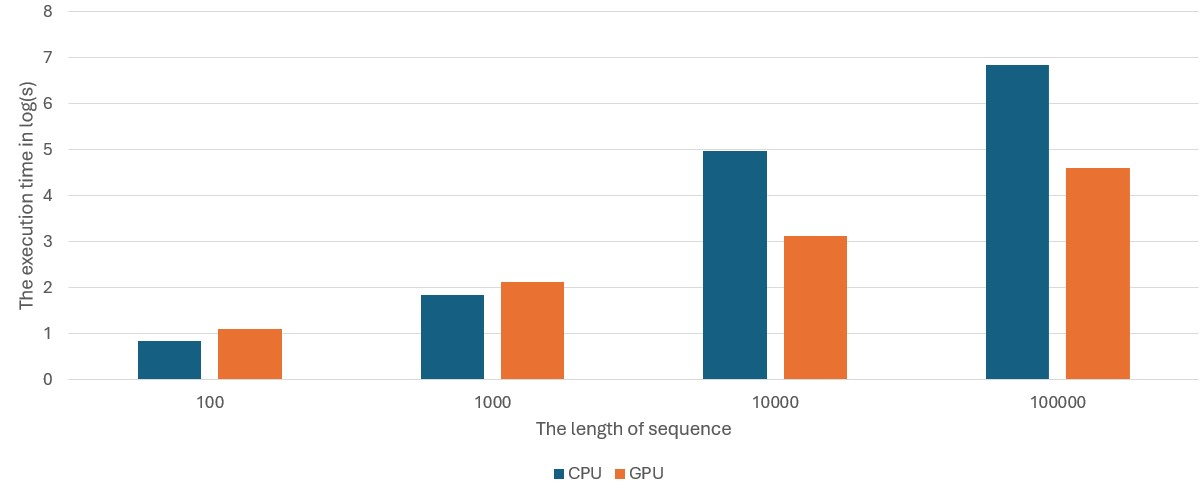
\includegraphics[width=1\linewidth]{figure/GPUCPU.jpg}
    \caption{The comparison of execution time with different sequence length}
    \label{fig:GPUCPU}
\end{figure}

\begin{figure}[h]
    \centering
    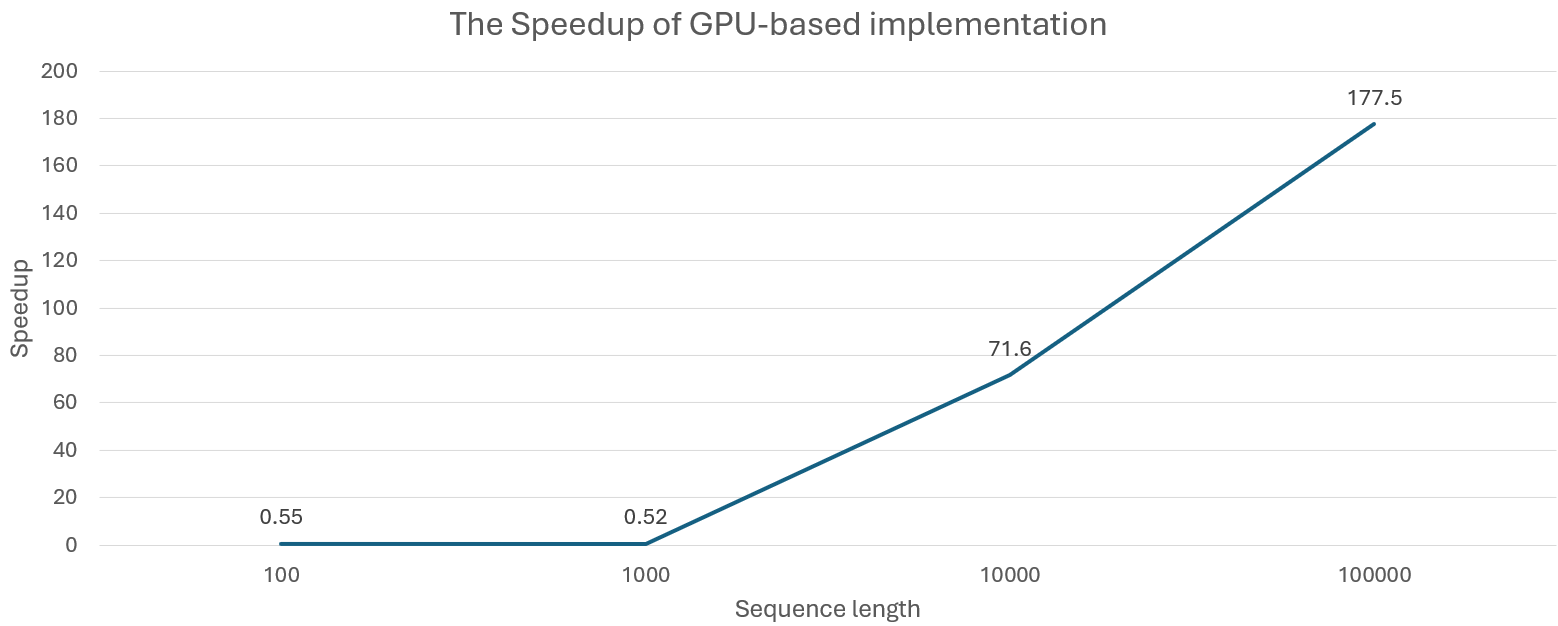
\includegraphics[width=0.9\linewidth]{figure/Speedup.png}
    \caption{The speedup of GPU-based implementation with different sequence length}
    \label{fig:speedup}
\end{figure}

\chapter{Discussion}
The results presented in this study demonstrate a significant improvement in computational efficiency when leveraging GPU-based acceleration of the Pair-HMM Forward Algorithm for DNA sequence profile, particularly for long sequence lengths. The GPU implementation significantly outperforms the CPU-based benchmark for the sequences longer than 10,000bp, showcasing the advantages of parallel processing capabilities inherent to GPU.

The speedup factor for sequences of 10,000 base pairs is approximately 71.6, while for sequences of 100,000bp, it is as high as 177.5. This indicates that the GPU-based implementation not only scales well with increasing sequence length but also becomes more efficient relative to the CPU-based approach as the data size grows.

However, the performance gain is not consistent across all sequence lengths. For shorter sequences, like 100 and 1,000bp, the GPU-based implementation is slower than the CPU-based benchmark. This difference is mainly because of the overhead linked to data transfer between the host and the device, which becomes a performance bottleneck for smaller datasets. The dynamic block technique also demonstrates varying effectiveness, providing significant advantages for longer sequences but introducing some overhead for shorter sequences.

For the configuration setting, the experiment reveals that there is no single best setting for all data. Settings need to be adjusted according to changes in data size. The block size of 32 with a thread size of 32 is the best configuration for a 100 and 1000bp sequence length, but it is the worst setting for a 10,000 and 100,000bp sequence length.

The results emphasize the importance of considering both computational workload and data transfer overhead when evaluating the performance of GPU-based implementations. For large-scale genomic data, the advantages of parallel computation on GPU surpass the overhead, leading to significant performance improvements. For smaller datasets, optimizing the data transfer process or using hybrid approaches may be necessary to achieve comparable performance gains.

\section{Future Work}
There are some future improvements we can try. 

(1) \textbf{Optimized Data Transfer}: One of the main bottlenecks in GPU-accelerated algorithms is the data transfer between the host (CPU) and the device (GPU). To mitigate this, we can use shared memory techniques to enable threads to communicate with each other, reducing the frequency and volume of data transfers. Additionally, employing strategies such as overlapping computation with data transfer can help hide the overhead, especially for short sequence sizes. This means we can initiate data transfers while computations are still ongoing, thus utilizing the GPU more effectively and reducing idle times.

(2) \textbf{Hybrid CPU-GPU Implementation}: Develop a hybrid approach that utilizes both CPU and GPU resources. For smaller sequences, the computation can be managed by the CPU to minimize data transfer overhead. This is because the cost of transferring data to the GPU might outweigh the benefits of parallel computation for short sequences. Conversely, longer sequences can be processed on the GPU, where the parallel processing capabilities can be fully utilized. By dynamically assigning tasks based on sequence length and complexity, we can achieve an optimal balance between CPU and GPU usage, improving overall efficiency and performance. In addition, developing an adaptive workload distribution algorithm that can dynamically adjust the allocation of tasks based on real-time performance metrics can further enhance the efficiency of this hybrid approach. This will ensure that the computational resources are utilized optimally, leading to faster and more efficient processing of DNA sequences.

\chapter{Conclusion}
In this paper, we present a GPU-accelerated implementation of the Pair-HMM Forward Algorithm for DNA sequence profile alignment, demonstrating substantial performance improvements over traditional CPU-based methods, particularly for long sequence lengths typical of TGS data. The use of anti-diagonal parallelization, anti-diagonal rolling, and dynamic block allocation significantly enhances the efficiency and scalability of the algorithm. However, for short NGS data, our approach suffers from data transfer overhead. We hope that shared memory techniques, overlapping data transfer overhead, and a hybrid approach could enhance the performance and applicability of the algorithms in the future. Additionally, our approach could serve as a considerable framework for those interested in the same field. They can customize it for their own goals, such as local alignment and gap score applications for the further research.
\newpage
\AddToContents{Bibliography}
\printbibliography


\end{document}
